\begin{tcolorbox}[colbacktitle=gray, title={\fontsize{35pt}{0pt}\selectfont 内部ノードにおける分割ルールの学習}]
	\structure{木探索(列挙木)} \\
	\vspace{10pt} \\
	全部分グラフ集合は{\bf \fontsize{26pt}{0pt}\selectfont 部分グラフ同型関係}により\\
	\express{木状探索空間}に表現が可能  \\
	\begin{textblock*}{\textwidth}(330pt,-100pt)
		\begin{figure}[h]
			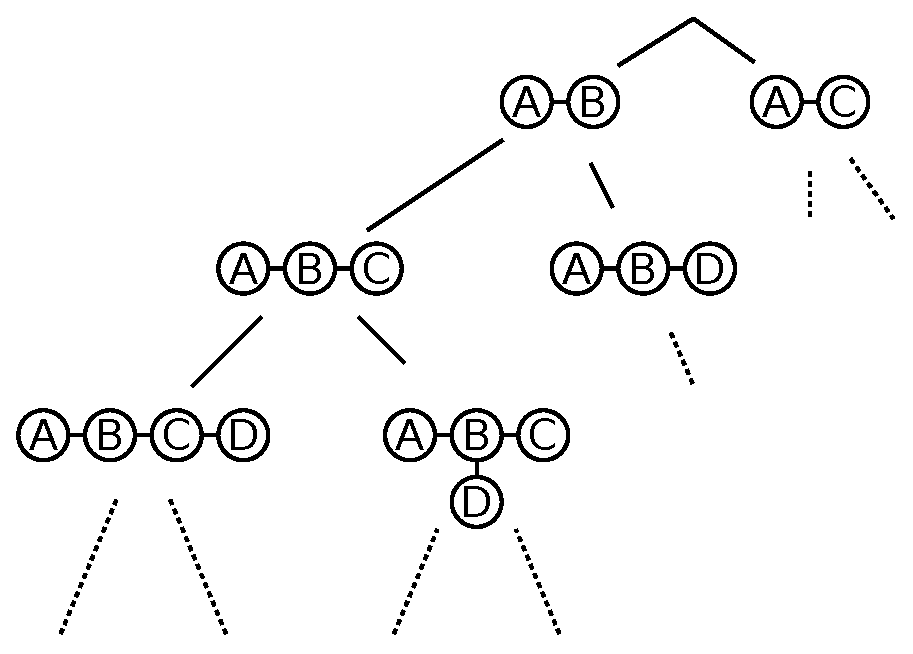
\includegraphics[width=0.4\hsize]{img/graph_search_tree.eps} \\
			\vspace{5pt}
			列挙木
		\end{figure}
	\end{textblock*}

	\vspace{100pt} 
	\structure{木探索の特性} \\
	\vspace{10pt}\\
	子ノード($c$)は親ノード($p$)の拡大グラフとなる \\ 
	\vspace{10pt}\\
	$~~~~~~~~~~~~~~~~~~~~~~~~~~ p \subset c$ \\
	\vspace{10pt}\\
	\hspace*{150pt} \includegraphics[width=0.5\graphwidth]{img/subgraph/kw.png}
	\hspace*{90pt} \includegraphics[width=0.7\graphwidth]{img/subgraph/kwg.png},
	\hspace*{-20pt} \includegraphics[width=0.7\graphwidth]{img/subgraph/kwy.png} \\
	\begin{textblock*}{\textwidth}(260pt,-30pt)
		$\subset$
	\end{textblock*}

	\vspace{10pt}
	$\rightarrow$ 子孫ノード$c$を含むグラフは常に親ノード$p$を含む \\
	$\rightarrow$ 子孫ノード$c$を含むグラフ集合は親ノード$p$を含むグラフ集合の部分集合となる \\
	%\vspace*{-20pt}
	\begin{equation}
		D_1(c) \subseteq D_1(p)
	\end{equation}

	\vspace*{15pt}
	\structure{最適部分グラフの探索} \\
	\vspace{10pt}\\
	- 列挙木の性質に基づいたBranch \& bound探索

	\vspace*{30pt}
	定理.\\
	$D_1(g)$と$D_0(g)$が与えられる時, $g' \supset g$を満たす全ての部分グラフに対して以下が成立
	\begin{eqnarray*}
		\TSS(D_1(g')) + \TSS(D_0(g')) \geq 
		\mymin{(\diamond,k)} \Big[\TSS(D_1(g) \setminus S_{\diamond, k}) + \TSS(D_0(g) \cup S_{\diamond, k}) \Big]
	\end{eqnarray*}
	$ (\diamond, k) \in \{ \leq, > \} \times \{ 2, \dots, |D_1(g) - 1| \} $,
	$S_{\diamond, k} \subset D_1(g)$,\\
	$S_{\leq, k}$は$D_1(g)$を残差に関して降順にした際の上から$k$番目までの集合.
	$S_{>, k}$は昇順.
\end{tcolorbox}
